\documentclass{beamer}
\usepackage[utf8]{inputenc}
\usepackage{latexsym,amsmath,xcolor,bm, amssymb, color, tikz, graphicx, amsthm, mathtools}
\usepackage{algorithm}
\usepackage{algorithmic}
\usepackage{hyperref}
\usepackage{float}     
\usepackage{CJKutf8}
\usepackage{multicol}

\graphicspath{{../logos/}}

\DeclareMathOperator*{\argmax}{arg\,max}
\DeclareMathOperator*{\argmin}{arg\,min}
\DeclareMathOperator{\sign}{sign}
\DeclareMathOperator{\Tr}{Tr}

\makeatletter
\DeclareRobustCommand\onedot{\futurelet\@let@token\@onedot}
\def\@onedot{\ifx\@let@token.\else.\null\fi\xspace}
\def\eg{\emph{e.g}\onedot} 
\def\Eg{\emph{E.g}\onedot}
\def\ie{\emph{i.e}\onedot} 
\def\Ie{\emph{I.e}\onedot}
\def\cf{\emph{c.f}\onedot} 
\def\Cf{\emph{C.f}\onedot}
\def\etc{\emph{etc}\onedot} 
\def\vs{\emph{vs}\onedot}
\def\wrt{w.r.t\onedot} 
\def\dof{d.o.f\onedot}
\def\etal{\emph{et al}\onedot}
\makeatother

\usetheme{Madrid}
\useinnertheme{circles}

\definecolor{ColorUNLP}{HTML}{8c0011} 
\usecolortheme[named=ColorUNLP]{structure}

%------------------------------------------------------------
\title{Bienvenidos al Training Camp Argentina 2026}
\subtitle{Acto de Apertura}
\author[AAPC]{Asociación Argentina de Programación Competitiva}
\institute[]{Universidad Nacional de La Plata -- Facultad de Informática}
\date[TC 2026]{Training Camp 2026}
\titlegraphic{
\includegraphics[clip,height=2cm,keepaspectratio]{logoTC.pdf}}
%------------------------------------------------------------

\AtBeginSection[]
{
  \begin{frame}
    \frametitle{Temario}
    \tableofcontents[currentsection]
  \end{frame}
}

\begin{document}

\frame{\titlepage}

% --- Sponsors Frame ---
\begin{frame}{Gracias Sponsors!}
    \begin{columns}[t]
        \column{0.5\textwidth}
        \centering
        Organiza\\
        \vspace{0.5cm}
        
\includegraphics[width=0.6\textwidth,keepaspectratio]{logo_aapc.png}\\
        \vspace{0.3cm}
        
\includegraphics[width=0.8\textwidth,keepaspectratio]{unlp_informatica.png}
        \column{0.5\textwidth}
        \centering
        Diamond Sponsor\\
        \vspace{0.5cm}
        
\includegraphics[width=0.8\textwidth,keepaspectratio]{GTSlogo.jpeg}
    \end{columns}
\end{frame}

\begin{frame}
\frametitle{Temario}
\tableofcontents
\end{frame}

\section{¿Qué es el Training Camp?}

\begin{frame}{¿Qué es el Training Camp?}
Es un entrenamiento intensivo de Programación Competitiva de 2 semanas:
\begin{itemize}
    \item \textbf{Teórico} (clases y discusión por la mañana) 
    \item \textbf{Práctico} (simulaciones de competencia por la tarde)
\end{itemize}
\vspace{0.3cm}
Entrenamos para prepararnos para las competencias de la ICPC.
\vfill
\centering

\includegraphics[clip,height=3cm,keepaspectratio]{icpc.jpeg}
\end{frame}

\section{El Camino de ICPC}

\begin{frame}{El Camino de ICPC}
    \centering
    
\includegraphics[clip,height=3cm,keepaspectratio]{icpc.jpeg}
    \vspace{0.5cm}
    
\begin{tikzpicture}[scale=0.95]
        \draw (1,0) -- (11,0);
        \foreach \x in {1, 4.2, 7.5, 11}
            \draw (\x cm,3pt) -- (\x cm,-3pt);
        
        \draw (1,0) node[above=4pt, align=center] {\small \textbf{Nacionales / TAP}}
                    node[below=4pt, align=center] {\small Ago/Sep};
        
        \draw (4.2,0) node[above=4pt, align=center] {\small \textbf{Regionales (SAS)}}
                      node[below=4pt, align=center] {\small Noviembre};
        
        \draw (7.5,0) node[above=4pt, align=center] {\small \textbf{PDA (Monterrey)}}
                      node[below=4pt, align=center] {\small Marzo};
        
        \draw (11,0) node[above=4pt, align=center] {\small \textbf{World Finals}}
                     node[below=4pt, align=center] {\small A definir};
    \end{tikzpicture}
\end{frame}

\section{Datos del TC}
\begin{frame}{Datos del TC}
    \begin{itemize}
        \item En estas dos semanas van a resolver entre \textbf{35 y 70 problemas}.
        \item Desde el 2010, el \textbf{95\%} de los finalistas argentinos del mundial de ICPC participaron del TC Argentina.
        \item De los últimos \textbf{6} equipos Campeones de América Latina (Latam Champions), \textbf{5} contaron con participantes del TC Argentina.
    \end{itemize}
\end{frame}

\section{Un poco de historia del TC}

\begin{frame}{Los comienzos}
    \begin{itemize}
        \item El Training Camp Argentina nace en \textbf{2010}, inspirándose en los entrenamientos que venían realizándose en Rusia, y que habían comenzado el año anterior en Brasil.
        \item Ese primer Training Camp duró 5 días y se realizó en la UBA.
        \item Ese primer año solo participaron equipos de Argentina.
        \item Ya al año siguiente se sumaron equipos de países vecinos de toda Latinoamérica.
    \end{itemize}
\end{frame}

\begin{frame}{Sedes Históricas}
    \begin{columns}
        \column{0.5\textwidth}
        \small
        \begin{itemize}
            \item 2010 - FCEN UBA, CABA
            \item 2011 - FCEN UBA, CABA
            \item 2012 - FAMAF UNC, Córdoba
            \item 2013 - UNLP, La Plata
            \item 2014 - FCEN UBA, CABA
            \item 2015 - UNS, Bahía Blanca
            \item 2016 - UNComa, Neuquén
            \item 2017 - UNSAM, San Martín
        \end{itemize}
        \column{0.5\textwidth}
        \small
        \begin{itemize}
            \item 2018 - FCEN UBA, CABA
            \item 2019 - FAMAF UNC, Córdoba
            \item 2020 - Remoto
            \item 2021 - Remoto
            \item 2022 - Remoto
            \item 2023 - UNLaM, La Matanza
            \item 2024 - UNR, Rosario
            \item 2025 - UTN-FRSF, Santa Fe
            \item $\bm{2026 - UNLP, La Plata}$
        \end{itemize}
    \end{columns}
\end{frame}

\section{Sede: Universidad Nacional de La Plata}

\begin{frame}{Universidad Nacional de La Plata}
    \centering
    
\includegraphics[width=0.8\textwidth]{unlp_informatica.png}
    \vspace{0.3cm}
    \begin{block}{Facultad de Informática}
        Referente en la formación y desarrollo científico en ciencias de la computación en la región, y sede recurrente de competencias de programación competitiva.
    \end{block}
\end{frame}

\begin{frame}{UNLP en ICPC World Finals}
    La UNLP cuenta con una trayectoria histórica destacada en las Finales Mundiales de ICPC:
    \vspace{0.2cm}
    \begin{columns}
        \column{0.55\textwidth}
        \begin{block}{Harbin, China 2010}
            \begin{itemize}
                \item \textbf{Equipo}: UN La Plata Ni JiRaFa
                \item \textbf{Integrantes}: Fidel Ivan Schaposnik, Joaquín Rodrigues, Ramiro Lafuente
                \item \textbf{Logro}: Puesto \textbf{45} a nivel mundial (4 problemas resueltos).
            \end{itemize}
        \end{block}
        
        \column{0.45\textwidth}
        \centering
        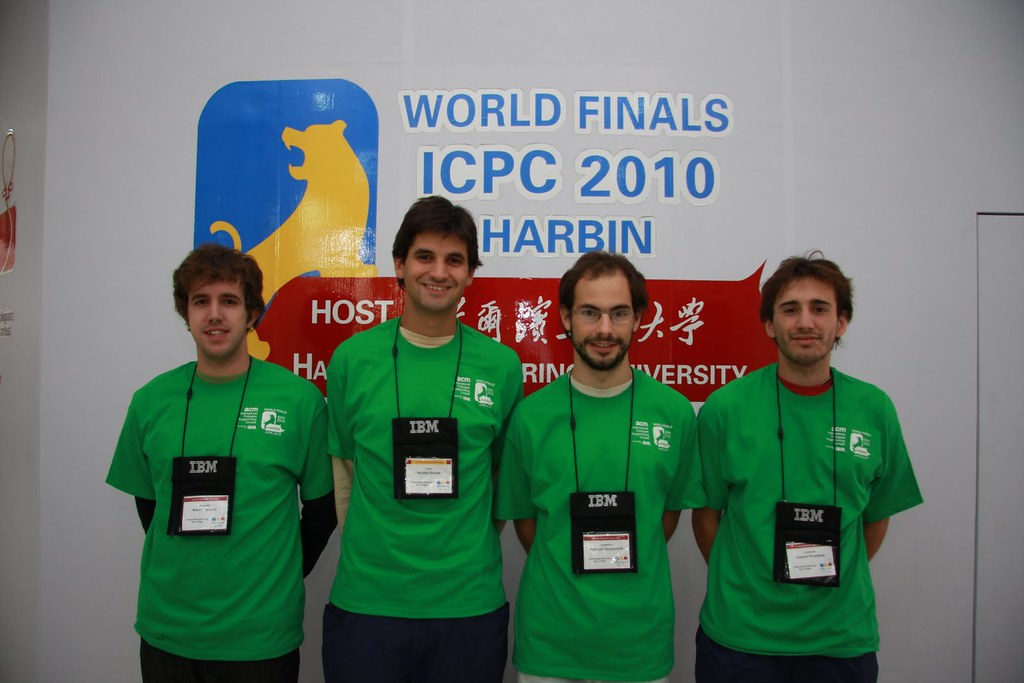
\includegraphics[width=\textwidth,keepaspectratio]{img/unlp_wf_2010.jpg}
    \end{columns}
\end{frame}

\begin{frame}{UNLP en ICPC World Finals}
    \begin{columns}
        \column{0.55\textwidth}
        \begin{block}{Baku, Azerbaiyán 2025}
            \begin{itemize}
                \item \textbf{Equipo}: NaN (Need a Name)
                \item \textbf{Logro}: Puesto \textbf{32} a nivel mundial -- \textbf{8°} lugar en América Latina (5 problemas resueltos).
            \end{itemize}
        \end{block}
        \vspace{0.1cm}
        \begin{block}{Dubai, Emiratos Árabes 2026}
            \begin{itemize}
                \item \textbf{Equipo}: NaN (Need a Name)
                \item \textbf{Logro}: Clasificados a la Final Mundial en Dubai (Noviembre 2026).
            \end{itemize}
        \end{block}
        
        \column{0.45\textwidth}
        \centering
        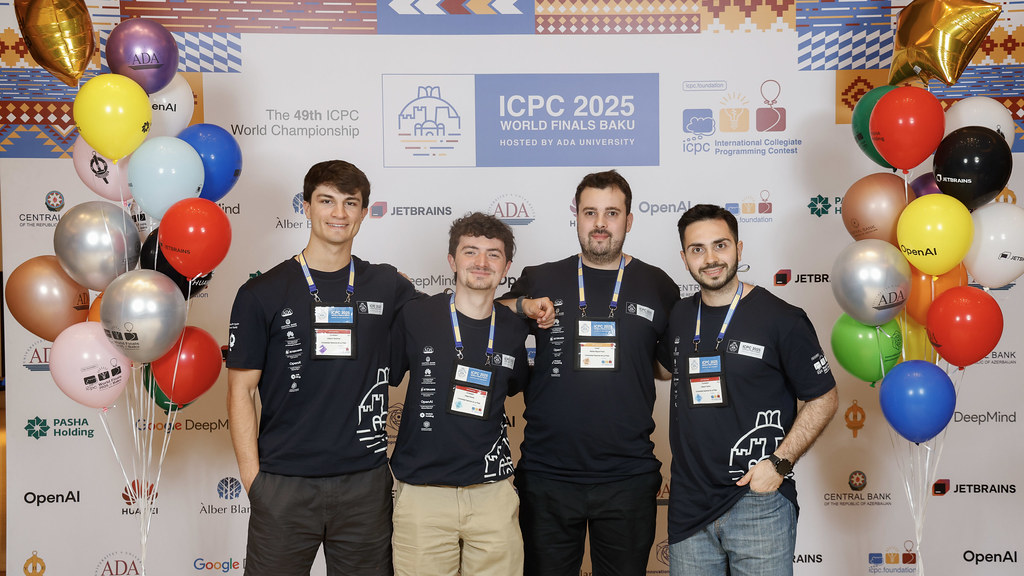
\includegraphics[width=\textwidth,keepaspectratio]{img/unlp_wf_2025.jpg}
    \end{columns}
\end{frame}

\section{Palabras}

\begin{frame}{Palabras de Bienvenida}
    \centering
    
\includegraphics[width=0.6\textwidth]{unlp_informatica.png}
    \vspace{0.5cm}
    \begin{itemize}
        \item \textbf{Dr. Marcelo Naiouf} -- Decano de la Facultad de Informática de la UNLP
        \item \textbf{[Representante de la AAPC]} -- Asociación Argentina de Programación Competitiva
    \end{itemize}
\end{frame}

\section{Cronograma}

\begin{frame}{Cronograma: Día Inaugural (20/07)}
    \begin{block}{Lunes 20 de Julio}
        \centering
        \begin{tabular}{|l|l|}
            \hline
            \textbf{Horario} & \textbf{Actividad} \\
            \hline
            08:30 a 09:30 & Acreditación (ingreso a la facultad) \\
            09:30 a 10:00 & Apertura del TC \\
            10:30 a 12:00 & Clases Teóricas (Inicial / Avanzado) \\
            12:00 a 13:30 & Almuerzo \\
            13:30 a 18:30 & Simulación de Competencia \\
            \hline
        \end{tabular}
    \end{block}
\end{frame}

\begin{frame}{Cronograma: Día GTS (21/07)}
    \begin{block}{Martes 21 de Julio}
        \centering
        \small
        \begin{tabular}{|l|l|}
            \hline
            \textbf{Horario} & \textbf{Actividad} \\
            \hline
            09:00 a 10:30 & Clases Teóricas (Inicial / Avanzado) \\
            10:30 a 11:00 & Coffee Break \\
            11:00 a 12:00 & Charla Apertura GTS \\
            12:00 a 13:30 & Almuerzo y foto grupal \\
            13:30 a 17:30 & Algorithmic Training Competition \\
            17:30 a 18:30 & Cierre y entrega de premios \\
            \hline
        \end{tabular}
    \end{block}
\end{frame}

\begin{frame}{Cronograma: Día Panel Pablo Heiber (22/07)}
    \begin{block}{Miércoles 22 de Julio}
        \centering
        \begin{tabular}{|l|l|}
            \hline
            \textbf{Horario} & \textbf{Actividad} \\
            \hline
            09:00 a 10:00 & Resolución de problemas \\
            10:00 a 10:30 & Coffee Break \\
            10:30 a 12:00 & Charla/Panel con Pablo Heiber \\
            12:00 a 13:30 & Almuerzo \\
            13:30 a 18:30 & Simulación de Competencia \\
            \hline
        \end{tabular}
    \end{block}
\end{frame}

\begin{frame}{Cronograma: Días Normales (23 al 30/07)}
    \begin{block}{Esquema Diario}
        \centering
        \begin{tabular}{|l|l|}
            \hline
            \textbf{Horario} & \textbf{Actividad} \\
            \hline
            09:00 a 10:00 & Resolución de problemas \\
            10:00 a 10:30 & Coffee Break \\
            10:30 a 12:00 & Clases Teóricas (Inicial / Avanzado) \\
            12:00 a 13:30 & Almuerzo \\
            13:30 a 18:30 & Simulación de Competencia \\
            \hline
        \end{tabular}
    \end{block}
\end{frame}

\begin{frame}{Cronograma: Día de Cierre (31/07)}
    \begin{block}{Viernes 31 de Julio}
        \centering
        \small
        \begin{tabular}{|l|l|}
            \hline
            \textbf{Horario} & \textbf{Actividad} \\
            \hline
            09:00 a 10:00 & Resolución de problemas \\
            10:00 a 10:30 & Coffee Break \\
            10:30 a 12:00 & Resolución de problemas \\
            12:00 a 13:30 & Almuerzo \\
            13:30 a 14:30 & Reunión de feedback y espacio de discusión \\
            14:30 a 15:30 & Entrega de Premios -- Cierre del TC \\
            \hline
        \end{tabular}
    \end{block}
\end{frame}

\begin{frame}{Almuerzo}
    \centering
    El almuerzo es de \textbf{12:00 a 13:30 hs}, el horario se respeta siempre.
    \vspace{0.3cm}
    \begin{alertblock}{¡No lleguen tarde!}
        El espacio y los tiempos son limitados. Seamos ordenados y respetemos las pautas indicadas por el staff de la sede.
    \end{alertblock}
    \vfill
    \textbf{*Seamos limpios*}
\end{frame}

\section{Aulas y espacios}

\begin{frame}{Aulas y Espacios de Trabajo}
    \begin{block}{Teoría y Práctica}
        \begin{itemize}
            \item \textbf{Clases Teóricas}: \textbf{[Aula de Teoría - A confirmar]}
            \item \textbf{Simulaciones (Práctica)}:
                \begin{itemize}
                    \item \textbf{[Laboratorio de Computación - A confirmar]}
                    \item Espacios habilitados para el uso de notebooks personales.
                \end{itemize}
        \end{itemize}
    \end{block}
    \vfill
    \small{Consulte con los voluntarios o mediante el grupo de Telegram para conocer las ubicaciones exactas dentro de la facultad.}
\end{frame}

\section{Dudas}

\begin{frame}{Dudas y Consultas}
    Ante cualquier duda o inconveniente durante el campamento:
    \vspace{0.4cm}
    \begin{itemize}
        \item Contactar a cualquier miembro del \textbf{Staff} (organizadores o voluntarios identificados).
        \item Consultar a través del canal oficial de \textbf{Telegram}.
    \end{itemize}
\end{frame}

\begin{frame}{Gracias}
    \centering
    {\Large ¡Gracias a todos por venir!}
    \vspace{1cm}
    
    ¡Muchos éxitos en la simulación de hoy y en las dos semanas de entrenamiento!
\end{frame}

\end{document}
